\section{Materials and methods}\label{sec:methods}

\subsection{Study area}\label{subsec:study-area}

The Ramis River basin is located in the high-Andean Altiplano of
southern Peru and drains towards Lake Titicaca. The basin is therefore
part of a closed lacustrine system in which river inflow, precipitation
and evaporation exert strong control on lake-level variability
\citep{cross2001late,condom2004transient,lima2025modeling}. Previous
regional studies show that the hydrology of the Titicaca system is
controlled mainly by rainfall and evapotranspiration variability,
whereas snowmelt, ice melt and net irrigation withdrawals have a
secondary role at the lake-basin scale \citep{lima2025modeling}. This
regional behaviour makes the Ramis basin a relevant test case for a
rainfall--runoff framework designed to combine process-based memory,
stochastic forcing and machine-learning correction.

The basin is characterized by high elevation, sparse hydroclimatic
monitoring and a strongly seasonal precipitation regime. Rainfall is
concentrated during the austral summer wet season, while the dry season
is associated with prolonged recession and low-flow persistence
\citep{condom2004transient,nauditt2017conceptual,lima2025modeling}.
Such hydroclimatic asymmetry is challenging for lumped conceptual
models because a single storage response may be unable to represent both
wet-season peaks and dry-season baseflow. It is also challenging for
purely data-driven models, which may learn strong seasonal correlations
without representing the storage mechanisms that maintain discharge
between rainfall events \citep{van2013influence,lees2021benchmarking}.
Daily discharge observations used in this study correspond to the
Puente Ramis gauging station operated by SENAMHI-Peru.

%% [AUTHOR ACTION BEFORE SUBMISSION]
%% Insert the official gauged drainage area, station coordinates, gauge
%% elevation and complete record period from SENAMHI/ANA metadata. These
%% details were not included in the evidence package used for this phase
%% and should not be inferred.

\subsection{Hydro-meteorological data and temporal protocol}
\label{subsec:data-protocol}

The modelling unit is a daily hydro-meteorological record composed of
precipitation ($P_t$), minimum and maximum temperature
($T_{\min,t}$ and $T_{\max,t}$), potential evapotranspiration
($PET_t$) and observed streamflow ($Q^{obs}_t$). The rainfall--runoff
core uses an effective precipitation input defined as
\begin{equation}
P^{eff}_t = \max(P_t - PET_t,\;0),
\label{eq:peff}
\end{equation}
which provides a non-negative approximation of the water available for
runoff generation after atmospheric demand has been accounted for.

All experiments follow the same chronological split. Model calibration
and ML training use data from 8~September~1991 to 31~December~2008,
whereas validation uses data from 8~January~2009 to 31~December~2020.
The final leaderboard is computed over the common validation
intersection of all experiments, comprising $n=4367$ daily samples. This
common-window design prevents unequal evaluation support across
physical, ML and hybrid configurations and is especially important for
experiments that require lagged predictors or sequence construction.

Temporal leakage was controlled at four levels. First, lagged predictors
were constructed only from present or past information. Second,
sequence samples were generated independently within the training and
validation partitions. Third, scalers and transformations used by ML
models were fitted exclusively on training data and then applied to
validation data. Fourth, flow-regime thresholds used for diagnostic
stratification were estimated from training observations only. These
controls follow the broader hydrological ML recommendation that model
selection and preprocessing must preserve temporal ordering
\citep{arsenault2022continuous,chen2013finding}. The corresponding
audit status is reported in Table~\ref{tab:reproducibility}.

\subsection{Lumped rainfall--runoff core}\label{subsec:physical-core}

Although the implementation workflow occasionally uses the term
``hydrodynamic'', the model evaluated here is a lumped stochastic
rainfall--runoff simulator, not a spatially distributed hydraulic or
hydrodynamic solver. The process-based component is therefore described
as a catchment-scale discharge-dynamics model. Its fast-flow state is
represented by the recurrence
\begin{equation}
x_t = \left(1 - \frac{\mu}{\lambda}\right)x_{t-1} + P^{eff}_t,
\label{eq:ramis-state}
\end{equation}
where $\mu>0$ and $\lambda>0$ regulate catchment memory and recession
stability. The parameter constraint $0<\mu/\lambda<1$ ensures a stable,
non-oscillatory memory factor.

The fast-flow discharge component is updated as
\begin{equation}
Q^{fast}_t = Q^{fast}_{t-1}
  - \frac{\mu}{\lambda}\,Q_0
    \left(\frac{\max(Q^{fast}_{t-1},0)}{Q_0}\right)^{2\mu-1}
  + \frac{\alpha_A}{\lambda}\,x_{t-1}
  + \sigma\,Q^{fast}_{t-1}\,\Delta L_t,
\label{eq:ramis-fast}
\end{equation}
where $Q_0$ is a reference discharge, $\alpha_A$ is an empirical
conversion factor, $\sigma$ controls stochastic amplitude and
$\Delta L_t$ is a stochastic increment. In deterministic experiments,
the stochastic term is inactive. Negative simulated discharge is clipped
to zero when non-negative physical post-processing is enabled.

The recurrence in Eqs.~\ref{eq:ramis-state}--\ref{eq:ramis-fast}
represents catchment-scale nonlinearity through aggregated storage
behaviour. This interpretation is consistent with recession analyses in
which nonlinear catchment response can emerge from heterogeneous linear
storage elements rather than from a single local nonlinear mechanism
\citep{harman2009power}. In this setting, the parameter $\mu$ acts as a
shape parameter controlling the effective recession behaviour of the
lumped storage system.

\subsection{Linear baseflow reservoir}\label{subsec:baseflow}

An optional linear reservoir is used to represent hydrological memory
beyond the fast-flow recurrence. This addition is motivated by previous
work in the Titicaca region showing that groundwater storage fluxes are
important for explaining seasonal runoff persistence and dry-season
baseflow \citep{nauditt2017conceptual}. The reservoir also provides a
controlled way to test whether adding a simple memory component improves
simulation skill before introducing stochastic perturbations or ML
correction.

Recharge to the baseflow store is proportional to effective
precipitation:
\begin{equation}
R_t = c_r\,\alpha_A\,P^{eff}_t,
\label{eq:recharge}
\end{equation}
where $c_r\in[0,1]$ is the recharge coefficient. Storage and baseflow
discharge then evolve as
\begin{align}
S_{b,t+1} &= \max\!\left(0,\;S_{b,t} + R_t - k_b S_{b,t}\right),
\label{eq:storage}\\
Q^{base}_t &= k_b\,S_{b,t},
\label{eq:qbase}
\end{align}
where $k_b\in[0.001,0.5]$ is the linear recession coefficient. The
total process-based discharge is
\begin{equation}
Q^{phys}_t = \max\!\left(Q^{fast}_t + Q^{base}_t,\;0\right).
\label{eq:qtotal}
\end{equation}
The baseflow component is activated in E1, E3 and all hybrid
configurations. Its isolated contribution is evaluated through the
E1--E0 and E3--E2 ablation contrasts.

\subsection{L\'{e}vy perturbations and Monte Carlo physical ensembles}
\label{subsec:levy}

Stochastic physical experiments inject $\alpha$-stable L\'{e}vy-type
increments into Eq.~\ref{eq:ramis-fast}. The perturbation is governed
by stability, skewness, location and scale parameters. Heavy-tailed
increments are used to represent episodic deviations from the smooth
lumped response, which is relevant in a highly seasonal basin where
rainfall inputs and streamflow errors are not expected to be Gaussian.
This design is consistent with hydrological ensemble studies showing
that uncertainty is not limited to the mean response but also involves
dispersion, asymmetry and tail behaviour
\citep{hong2006uncertainty,gabellani2007propagation,abaza2017incidence}.

For each calibrated stochastic configuration, a Monte Carlo ensemble of
$N$ trajectories is generated. At each day, the ensemble is summarized
by central-tendency, dispersion and quantile descriptors. The quantile
set used in the hybrid experiments is
\begin{equation}
\{q_{0.01},\;q_{0.05},\;q_{0.25},\;q_{0.50},\;q_{0.75},
  \;q_{0.95},\;q_{0.99}\},
\label{eq:quantiles}
\end{equation}
together with spread measures such as $q_{0.95}-q_{0.05}$ and
$q_{0.75}-q_{0.25}$. Quantile representations are robust summaries of
non-Gaussian and fat-tailed distributions, and therefore provide a
natural way to pass distributional information from a stochastic
physical ensemble to an ML emulator \citep{swiderski2016aggregation}.
In this study, the same ensemble is evaluated in two roles: as a direct
stochastic physical predictor in E2 and E3, and as a source of
physically informed ML features in E5--E8.

\subsection{Machine-learning emulators and feature sets}
\label{subsec:emulator}

The ML component maps a feature vector $\mathbf{z}_t$ to daily simulated
discharge,
\begin{equation}
\hat{Q}_t = f_\theta(\mathbf{z}_t),
\label{eq:emulator}
\end{equation}
followed by non-negative clipping,
\begin{equation}
Q^{sim}_t = \max(\hat{Q}_t,\;0).
\label{eq:ml-clipping}
\end{equation}
This post-processing step ensures physically admissible discharge
predictions while preserving the fitted ML response over positive
flows.

Three feature families are compared. The pure ML baseline (E4) uses
observed hydro-meteorological forcings and non-negative lags, including
lagged runoff information where allowed by the temporal protocol.
Including antecedent runoff is hydrologically meaningful because it
acts as a proxy for catchment storage and has been shown to improve
rainfall--runoff ML models relative to meteorological predictors alone
\citep{adnan2021comparison}. Mean-based hybrids (E5 and E7) use the
mean trajectory of the stochastic physical ensemble. Quantile-based
hybrids (E6 and E8) use the ensemble quantiles and spread descriptors
listed in Eq.~\ref{eq:quantiles}. This design tests whether the ML
emulator benefits primarily from a corrected central physical trajectory
or from richer distributional descriptors of the physical ensemble.

The tabular emulator is labelled as XGB in the experiment names. In the
current evidence package, however, the actual backend was
\texttt{HistGradientBoostingRegressor} from scikit-learn, reported in
the audit tables as \texttt{sklearn\_hgb}. The corresponding results
are therefore interpreted as gradient-boosted tree hybrids rather than
as package-specific evidence for \texttt{xgboost}. Hyperparameter search
used temporally ordered cross-validation, avoiding random shuffling of
time steps during model selection.

The sequential emulator is labelled as GRU in the experiment names and
is designed to use recurrent layers when a supported backend is
available. In the present execution, the recurrent backend was not
available; the implementation flattened each input sequence and trained
a multilayer perceptron instead. Consequently, E7 and E8 are retained in
the experimental matrix because they evaluate sequentially constructed
features, but they are interpreted throughout the manuscript as
GRU-labelled fallback-MLP runs, not as evidence of true recurrent GRU
superiority \citep{kratzert2018rainfall,kratzert2019towards}.

\subsection{Calibration objective}\label{subsec:calibration}

The process-based and stochastic configurations are calibrated with a
scalar objective that combines efficiency, distributional agreement,
bias and interval coverage:
\begin{equation}
J = \frac{w_{NSE}(1-NSE) + w_{KGE}(1-KGE)
  + w_{PBIAS}\left|\frac{PBIAS}{100}\right|
  + w_{cov}|c^*-PICP|}{w_{active}},
\label{eq:objective}
\end{equation}
where $c^*=0.95$ is the nominal coverage target and $w_{active}$ is the
sum of the active weights. The default weights are $w_{NSE}=0.40$,
$w_{KGE}=0.30$, $w_{PBIAS}=0.15$ and $w_{cov}=0.15$. When a model does
not produce prediction intervals, the coverage term is omitted and the
remaining weights are renormalized.

The composite objective is used because no single deterministic metric
fully describes hydrological model performance, particularly when both
high-flow peaks and low-flow persistence are relevant
\citep{pushpalatha2012review}. The coverage term is included to avoid
selecting stochastic configurations that are sharp but severely
underdispersive, a common limitation in hydrological ensemble
prediction \citep{franz2011evaluating,abaza2017incidence}.

\subsection{Experimental matrix and ablation design}\label{subsec:matrix}

The experimental matrix was designed to isolate the contribution of each
modelling component under a common validation window. E0 and E1 compare
the deterministic RAMIS core without and with the baseflow reservoir.
E2 and E3 add L\'{e}vy stochasticity without and with baseflow. E4 is a
pure ML baseline trained only from observed predictors. E5 and E6 are
gradient-boosting hybrids using, respectively, ensemble-mean and
ensemble-quantile physical descriptors. E7 and E8 use the same mean and
quantile feature families in a sequential-feature setting, but with the
fallback MLP backend described above.

\begin{table*}[t]
\caption{Controlled experimental matrix. Backend entries report the
actual backend used in the current evidence package.}
\label{tab:experiment-matrix}
\centering
\small
\begin{tabular*}{\textwidth}{@{\extracolsep{\fill}}lllllll@{}}
\toprule
Experiment & Family & L\'{e}vy & Baseflow & Emulator & Features
  & Backend used \\
\midrule
E0\_RAMIS\_DET\_NOBF   & physical RAMIS & no  & no  & none
  & physical only & physical \\
E1\_RAMIS\_DET\_BF     & physical RAMIS & no  & yes & none
  & physical only & physical \\
E2\_RAMIS\_LEVY\_NOBF  & RAMIS--L\'{e}vy & yes & no  & none
  & physical only & physical \\
E3\_RAMIS\_LEVY\_BF    & RAMIS--L\'{e}vy & yes & yes & none
  & physical only & physical \\
E4\_ML\_PURE\_XGB      & pure ML        & no  & no  & XGB-labelled
  & observed forcings & sklearn\_hgb \\
E5\_HYB\_XGB\_MEAN     & hybrid         & yes & yes & XGB-labelled
  & ensemble mean & sklearn\_hgb \\
E6\_HYB\_XGB\_QUANTILES & hybrid        & yes & yes & XGB-labelled
  & ensemble quantiles & sklearn\_hgb \\
E7\_HYB\_GRU\_MEAN     & sequential hybrid & yes & yes & GRU-labelled
  & mean sequence & fallback MLP \\
E8\_HYB\_GRU\_QUANTILES & sequential hybrid & yes & yes & GRU-labelled
  & quantile sequence & fallback MLP \\
\bottomrule
\end{tabular*}
\end{table*}

This matrix supports five planned contrasts: the effect of baseflow
(E1--E0 and E3--E2), the direct effect of stochastic perturbations under
baseflow (E3--E1), the effect of pure ML correction relative to the full
stochastic physical model (E4--E3), the effect of hybridization
(E5--E3 and E6--E3), and the value of quantile descriptors relative to
mean descriptors (E6--E5 and E8--E7). The same validation samples are
used in every contrast.

\subsection{Relation to prior stochastic physical--ML hybridization}
\label{subsec:relation}

The idea of feeding descriptors from a stochastic physical ensemble into
an ML emulator is closely related to the hybridization strategy of
\citet{houenafa2025hybridization}. The present study is framed as an
ablation and audit extension of that idea. Rather than reporting only
the best hybrid configuration, it decomposes the pipeline into physical
memory, stochastic perturbation, ML correction and descriptor choice. It
also evaluates whether the same ensemble that improves ML features can
serve as a calibrated predictive uncertainty band. This distinction is
important because physically plausible ensemble spread does not
necessarily imply reliable probabilistic coverage
\citep{atger1999skill,franz2011evaluating,papacharalampous2022review}.

\subsection{Evaluation metrics and audit protocol}\label{subsec:evaluation}

Point-prediction performance is evaluated with Nash--Sutcliffe
efficiency (NSE), Kling--Gupta efficiency (KGE), root mean squared error
(RMSE), mean absolute error (MAE), percent bias (PBIAS) and the
coefficient of determination ($R^2$). Regime-specific metrics are
computed for low, mid and high flows using thresholds estimated from
training observations only. Low-flow NSE is interpreted cautiously
because efficiency scores based on squared error are sensitive to low
observed variance and can penalize dry-season errors in ways that are
not proportional to their hydrological relevance
\citep{pushpalatha2012review}.

Stochastic reference bands are evaluated using prediction interval
coverage probability (PICP), prediction interval normalized average
width (PINAW), mean prediction interval width (MPIW) and Winkler score.
The intended behaviour is high coverage with the narrowest possible
intervals, but sharpness is not interpreted as skill when coverage is
far below the nominal level \citep{franz2011evaluating,abaza2017incidence,papacharalampous2022review}.
The final audit checks chronological split integrity, feature
construction, target leakage, backend metadata, common-window
consistency and non-negative post-processing. The audit results are
reported in Table~\ref{tab:reproducibility}.

\begin{figure*}[t]
\centering
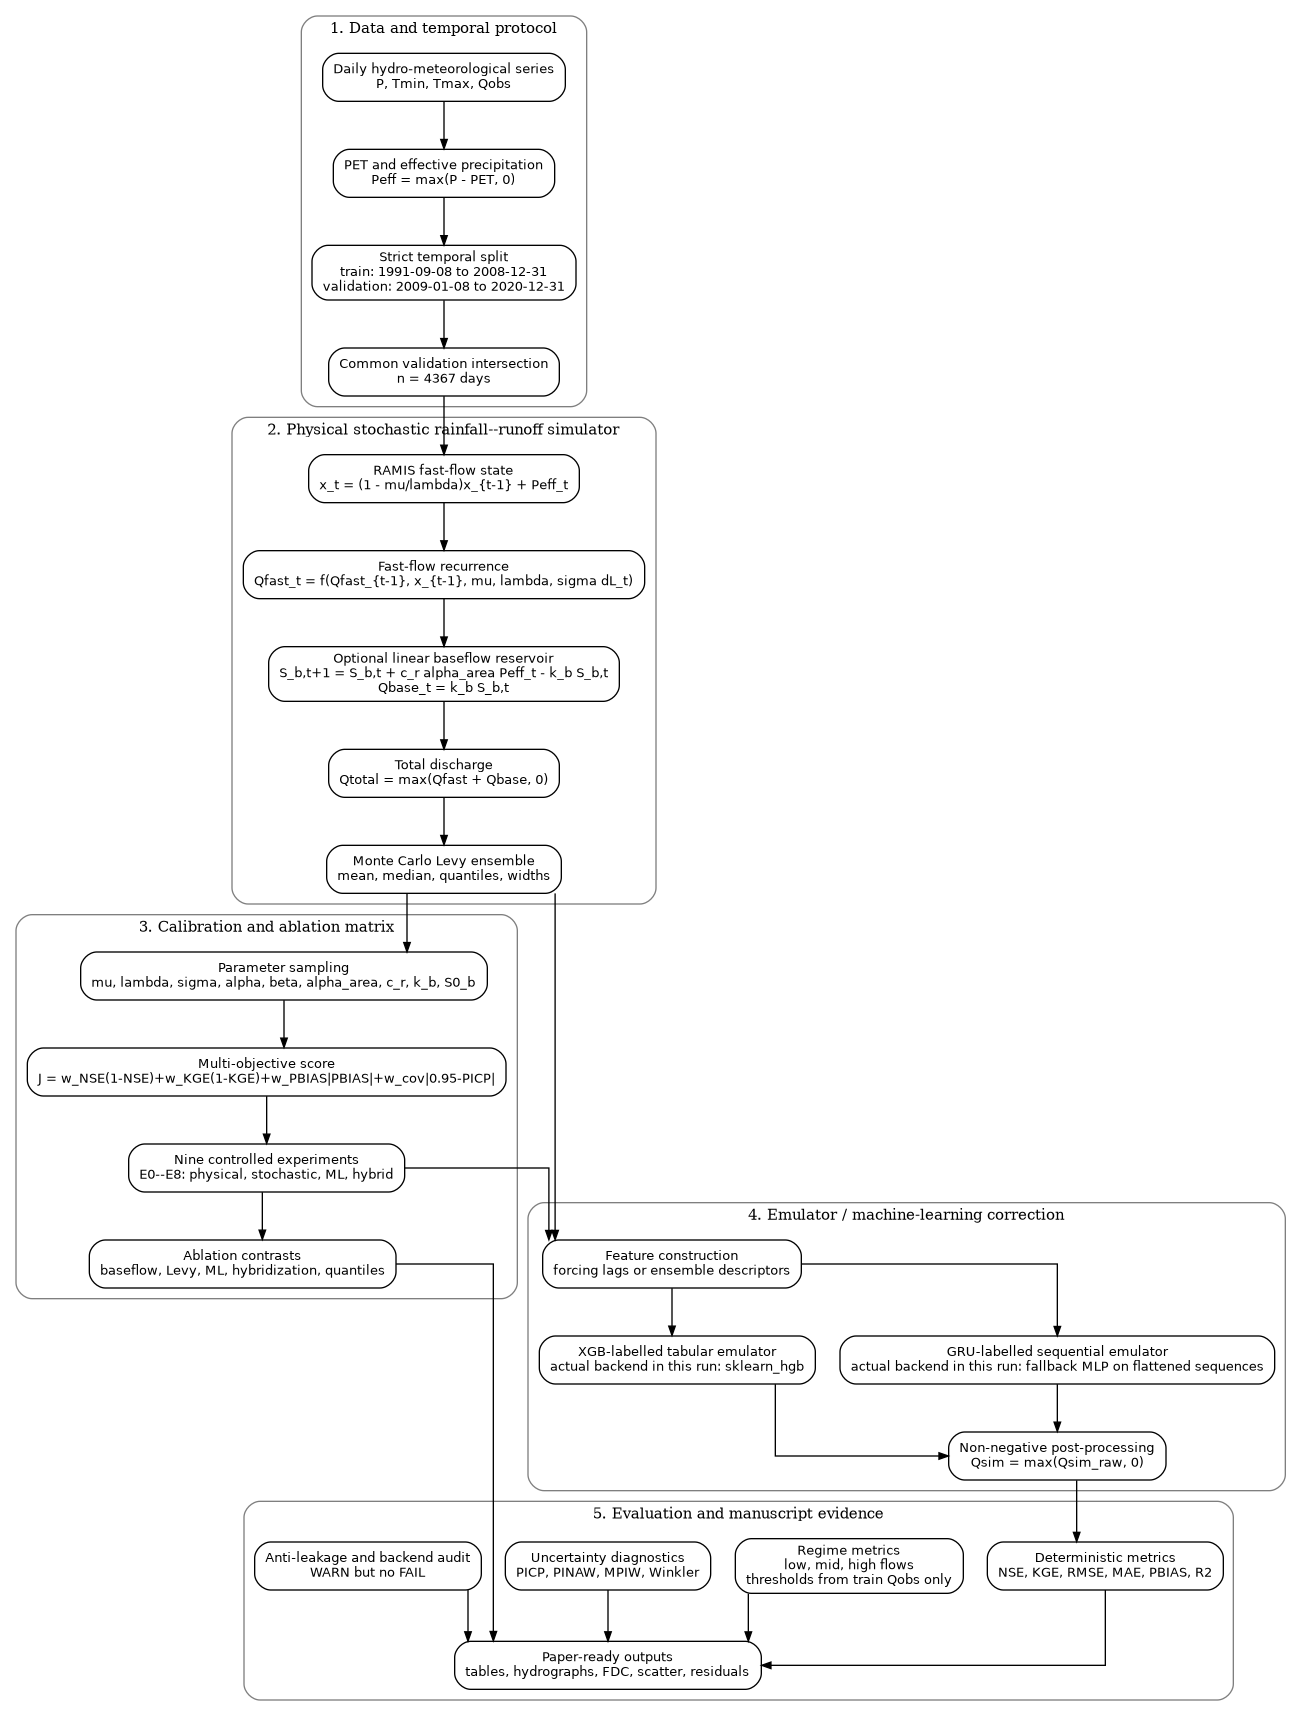
\includegraphics[width=0.96\textwidth]{figures/method_workflow.png}
\caption{StoHyMoLAP workflow from daily hydro-meteorological data to
lumped physical simulation, L\'{e}vy-type stochastic ensemble
generation, ensemble-descriptor construction, ML emulation, ablation
comparison and audit-controlled manuscript evidence.}
\label{fig:method-workflow}
\end{figure*}

%% =====================================================================
%% 3. RESULTS
%% =====================================================================
